% Diagram: Traditional vs Paged KV Cache Memory
% Shows memory fragmentation problem and how PagedAttention solves it

\begin{figure}[htbp]
\centering
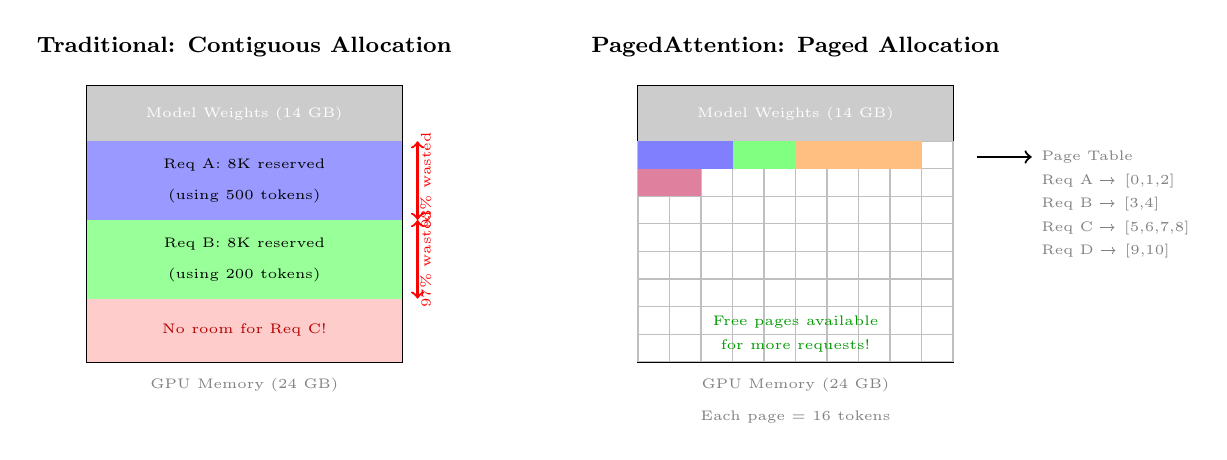
\begin{tikzpicture}[
    node distance=0.2cm,
    memblock/.style={rectangle, draw, minimum height=0.5cm, font=\tiny},
    label/.style={font=\footnotesize},
    timelabel/.style={font=\tiny, text=gray}
]

% === TRADITIONAL ALLOCATION (left) ===
\node[label] at (2, 4) {\textbf{Traditional: Contiguous Allocation}};

% GPU Memory block
\draw[thick] (0, 0) rectangle (4, 3.5);
\node[timelabel] at (2, -0.3) {GPU Memory (24 GB)};

% Model weights (fixed)
\fill[gray!40] (0, 2.8) rectangle (4, 3.5);
\node[font=\tiny, white] at (2, 3.15) {Model Weights (14 GB)};

% KV Cache allocations (pre-allocated for max length)
\fill[blue!40] (0, 1.8) rectangle (4, 2.8);
\node[font=\tiny] at (2, 2.5) {Req A: 8K reserved};
\node[font=\tiny] at (2, 2.1) {(using 500 tokens)};

\fill[green!40] (0, 0.8) rectangle (4, 1.8);
\node[font=\tiny] at (2, 1.5) {Req B: 8K reserved};
\node[font=\tiny] at (2, 1.1) {(using 200 tokens)};

% Wasted space indicator
\fill[red!20] (0, 0) rectangle (4, 0.8);
\node[font=\tiny, red!70!black] at (2, 0.4) {No room for Req C!};

% Fragmentation arrows
\draw[<->, red, thick] (4.2, 1.8) -- (4.2, 2.8);
\node[timelabel, red, rotate=90, anchor=south] at (4.5, 2.3) {93\% wasted};

\draw[<->, red, thick] (4.2, 0.8) -- (4.2, 1.8);
\node[timelabel, red, rotate=90, anchor=south] at (4.5, 1.3) {97\% wasted};

% === PAGED ATTENTION (right) ===
\node[label] at (9, 4) {\textbf{PagedAttention: Paged Allocation}};

% GPU Memory block
\draw[thick] (7, 0) rectangle (11, 3.5);
\node[timelabel] at (9, -0.3) {GPU Memory (24 GB)};

% Model weights (fixed)
\fill[gray!40] (7, 2.8) rectangle (11, 3.5);
\node[font=\tiny, white] at (9, 3.15) {Model Weights (14 GB)};

% Page pool - small fixed-size blocks
\foreach \i in {0,1,2,3,4,5,6,7} {
    \foreach \j in {0,1,2,3,4,5,6,7,8,9} {
        \pgfmathsetmacro{\x}{7 + \j * 0.4}
        \pgfmathsetmacro{\y}{0 + \i * 0.35}
        \draw[gray!50] (\x, \y) rectangle (\x + 0.4, \y + 0.35);
    }
}

% Color used pages
% Req A pages (blue) - scattered
\fill[blue!50] (7, 2.45) rectangle (7.4, 2.8);
\fill[blue!50] (7.4, 2.45) rectangle (7.8, 2.8);
\fill[blue!50] (7.8, 2.45) rectangle (8.2, 2.8);

% Req B pages (green) - scattered
\fill[green!50] (8.2, 2.45) rectangle (8.6, 2.8);
\fill[green!50] (8.6, 2.45) rectangle (9.0, 2.8);

% Req C pages (orange) - can now fit!
\fill[orange!50] (9.0, 2.45) rectangle (9.4, 2.8);
\fill[orange!50] (9.4, 2.45) rectangle (9.8, 2.8);
\fill[orange!50] (9.8, 2.45) rectangle (10.2, 2.8);
\fill[orange!50] (10.2, 2.45) rectangle (10.6, 2.8);

% Req D pages (purple)
\fill[purple!50] (7, 2.1) rectangle (7.4, 2.45);
\fill[purple!50] (7.4, 2.1) rectangle (7.8, 2.45);

% Free pages indicator
\node[timelabel, green!60!black] at (9, 0.5) {Free pages available};
\node[timelabel, green!60!black] at (9, 0.2) {for more requests!};

% Legend
\node[timelabel] at (9, -0.7) {Each page = 16 tokens};

% Page table concept
\draw[->, thick] (11.3, 2.6) -- (12, 2.6);
\node[timelabel, anchor=west] at (12, 2.6) {Page Table};
\node[timelabel, anchor=west, font=\tiny] at (12, 2.3) {Req A → [0,1,2]};
\node[timelabel, anchor=west, font=\tiny] at (12, 2.0) {Req B → [3,4]};
\node[timelabel, anchor=west, font=\tiny] at (12, 1.7) {Req C → [5,6,7,8]};
\node[timelabel, anchor=west, font=\tiny] at (12, 1.4) {Req D → [9,10]};

\end{tikzpicture}
\caption{Traditional vs PagedAttention memory management. Left: Contiguous allocation reserves maximum possible space per request, causing fragmentation and limiting concurrent requests. Right: PagedAttention allocates small fixed-size pages on demand, eliminating fragmentation and enabling 2-4x more concurrent requests.}
\label{fig:paged-attention}
\end{figure}
